% A reference card for the darktable photography workflow application.
% Copyright (C) 2015 Mark Richters

\RequirePackage[l2tabu,orthodox]{nag}
\documentclass[\ArgLang,\ArgFormat,9pt]{extarticle}
\usepackage[utf8]{inputenc}
\usepackage[T1]{fontenc}
\usepackage{babel}
\usepackage{textcomp}
%\usepackage{helvet}
\usepackage{newcent}
\usepackage[landscape,margin={1cm,2cm}]{geometry}
\usepackage{microtype}
\usepackage{multicol}
\usepackage{graphicx}
\usepackage{color}
\usepackage{tabularx}
\usepackage{fancyhdr}

% i18n

\input {lang-\ArgLang}

\usepackage[hidelinks,pdftex,pdfauthor={Mark Richters},pdftitle={\LANGDarktableRefcard},pdfkeywords={darktable}]{hyperref}

\graphicspath{{images/},{images-modules/}}

\pagestyle{fancy}

% background and text colors

\input {color-\ArgColor}

\parindent0em
\sloppy

% Header
\fancyhead{}
\fancyfoot{}

\lhead{\color{textcol}\LARGE\bfseries
\includegraphics[height=1\baselineskip]{darktable} \raisebox{.35\height}{\LANGDarktableRefcard}}

\lfoot{\color{textcol}\tiny\ \copyright\ 2015 Mark Richters. \raisebox{-.15\height}{
\includegraphics[height=1em]{license}} This work is licensed under a Creative Commons Attribution-ShareAlike 4.0 International License (\href{http://creativecommons.org/licenses/by-sa/4.0/}{http://creativecommons.org/licenses/by-sa/4.0/}). \hfill v\ArgVersion}

\renewcommand{\headrulewidth}{0.4pt}
\renewcommand{\headrule}{{\color{red}\hrule width\headwidth height\headrulewidth \vskip-\headrulewidth}}
\renewcommand{\footrulewidth}{0pt}
\renewcommand{\footrule}{{\color{keycol}\vskip-\footruleskip\vskip-\footrulewidth\hrule width\headwidth height\footrulewidth\vskip\footruleskip}}


% Change font

\renewcommand{\familydefault}{\sfdefault}

% No section numbers

\setcounter{secnumdepth}{0}

% style for keyboard shortcuts in tables

\newcolumntype{k}{>{\bfseries}r<{}}

\setlength{\columnseprule}{1pt}
\renewcommand{\columnseprulecolor}{\color{sepcol}}

\begin{document}

\pagecolor{pagecol}
\color{textcol}

\begin{multicols}{3}
  \newlength{\tabwidth}
  \setlength{\tabwidth}{0.975\linewidth}

%  \raggedcolumns
  \raggedright

  \section{\LANGGlobalShortcuts}
  
  \subsection{\LANGSwitchingViews}

  \colorbox{keycol}{%
    \begin{tabularx}{\tabwidth}{k@{ -- }X} 
      l & \LANGLighttable \\
      d & \LANGDarkroom \\
      t & \LANGCameraTethering \\
      m & \LANGMap \\
      s & \LANGSlideshow \\
      . & \LANGSwitchView \\
      \LANGCtrl-q & \LANGQuitDarktable \\
    \end{tabularx}}
  
  \subsection{\LANGBrightnessAndContrast}

  \colorbox{keycol}{%
    \begin{tabularx}{\tabwidth}{k@{ -- }X} 
      F7 & \LANGDecreaseContrast \\
      F8 & \LANGIncreaseContrast \\
      F9 & \LANGDecreaseBrightness \\
      F10 & \LANGIncreaseBrightness 
    \end{tabularx}}
  
  \subsection{\LANGChangingViews}

  \colorbox{keycol}{%
    \begin{tabularx}{\tabwidth}{k@{ -- }X} 
      F11 & \LANGToggleFullscreen \\
      \LANGEsc & \LANGLeaveFullscreen \\
      \LANGCtrl-h & \LANGToggleHeader \\
      \LANGTab & \LANGToggleSideBorders \\
      \LANGCtrl-f & \LANGToggleFilmStrip\ \raisebox{-.25\height}{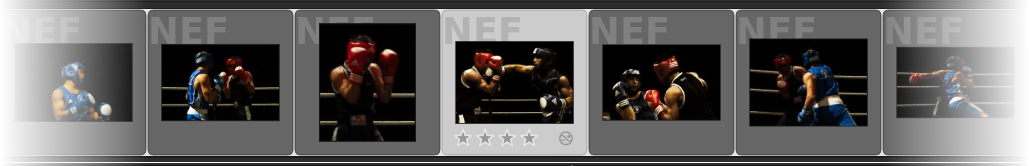
\includegraphics[height=1em]{filmstrip}} \\
    \end{tabularx}}

  \section{\LANGLighttable}

  \colorbox{keycol}{%
    \begin{tabularx}{\tabwidth}{k@{ -- }X} 
      0 -- 5 & \LANGRateImageWithStars\ \raisebox{-.15\height}{
\includegraphics[height=1em]{star_rating_panel}} \\
      r & \LANGRejectImage \\
      F1 -- F5 & \LANGAssignColorLabel\ \raisebox{-.15\height}{
\includegraphics[height=1em]{color_labels_panel}} \\
      \LANGCtrl-c & \LANGCopyHistoryStack \\
      \LANGCtrl-v & \LANGPasteHistoryStack \\ 
      d & \LANGOpenInDarkroom \\
      z & \LANGZoomIntoImage \\
      \LANGCtrl-z & \LANGZoomAndShowFocusAreas \\
      \LANGCtrl-g & \LANGGroupImages \\
      \LANGShift-\LANGCtrl-g & \LANGUngroupImages \\
      \LANGCtrl-t & \LANGTag \\
      \LANGCtrl-e & \LANGExport 
    \end{tabularx}}

  \section{\LANGSlideshow}

  \colorbox{keycol}{%
    \begin{tabularx}{\tabwidth}{k@{ -- }X}
      \LANGLeftClick & \LANGNextImage \\
      \LANGRightClick & \LANGPreviousImage \\
      \LANGSpace & \LANGStartStop \\
      \LANGEsc & \LANGExitSlideshow \\
    \end{tabularx}}
  
  \bigskip

  \begin{center}
    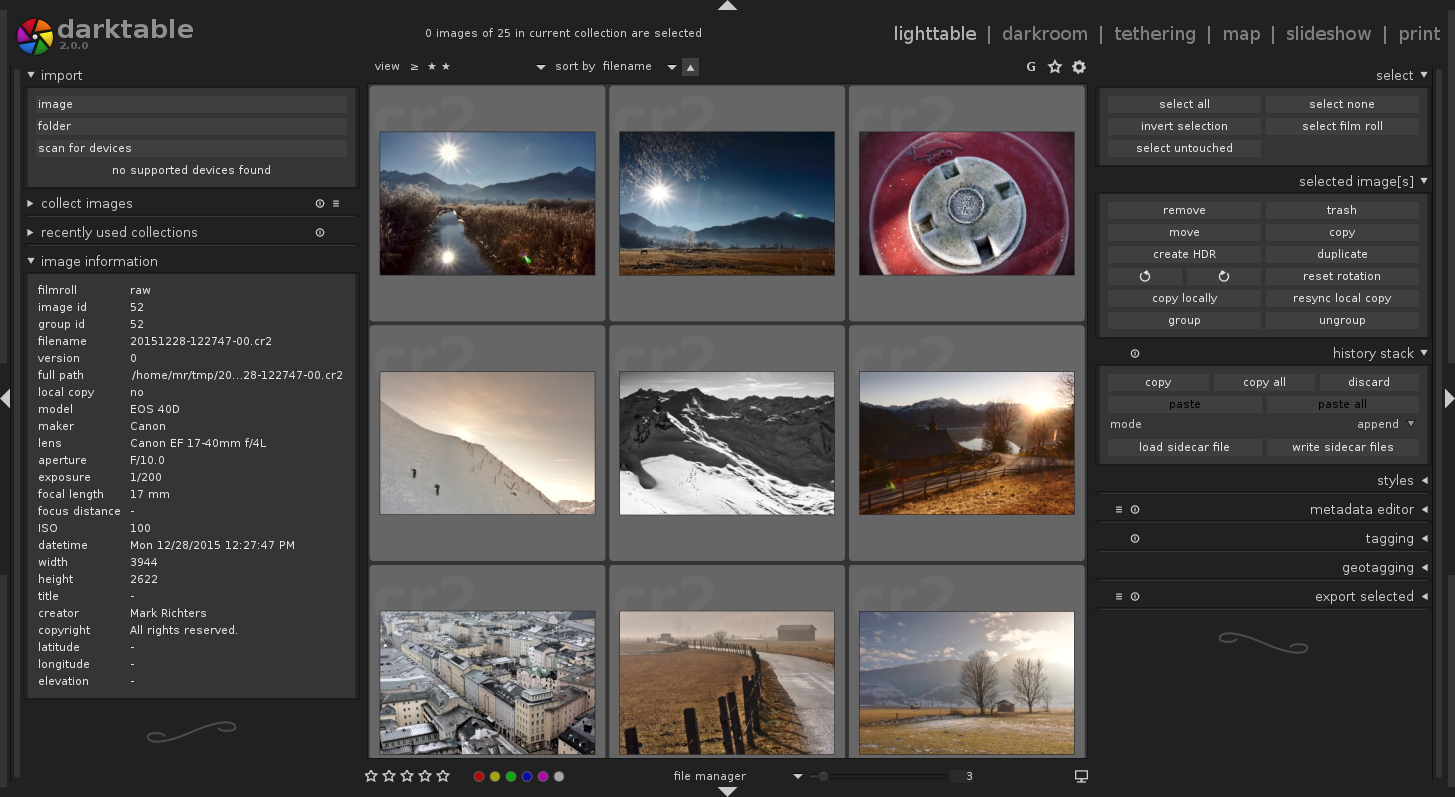
\includegraphics[height=5.5em]{lighttable_view2}
    \qquad
    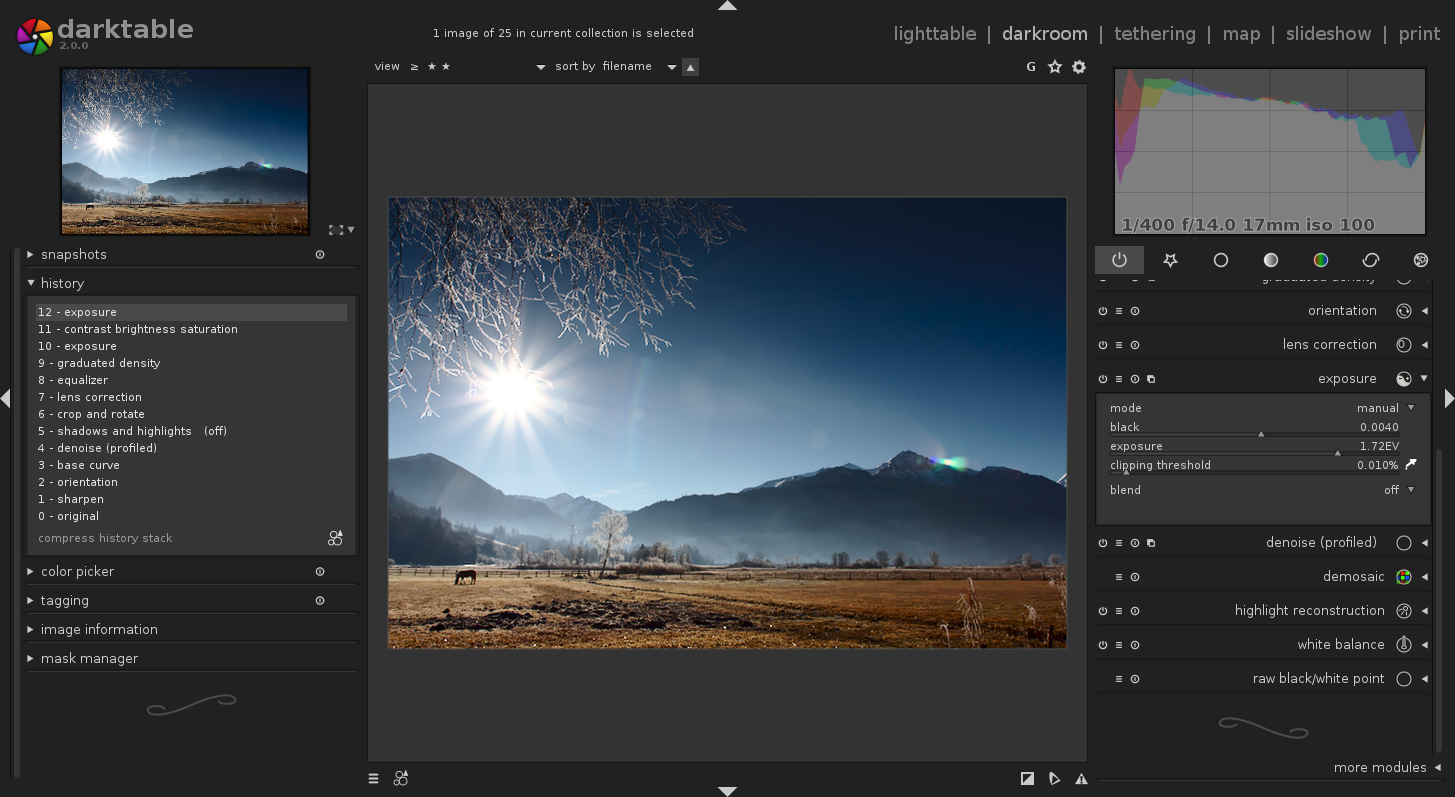
\includegraphics[height=5.5em]{darkroom_view2}
  \end{center}
  
  \section{\LANGDarkroom}

  \colorbox{keycol}{%
    \begin{tabularx}{\tabwidth}{k@{ -- }X} 
      c & \LANGCompressHistoryStack \\
      o & \LANGOverUnderexposed \\
      \LANGCtrl-e & \LANGExport \\
      \LANGSpace & \LANGNextImage \\
      \LANGBackspace & \LANGPreviousImage \\
      \mbox{]} & \LANGBrushLarger \\
      \mbox{[} & \LANGBrushSmaller \\
      \LANGAlt-1 & \LANGZoomCloseUp \\
      \LANGAlt-2 & \LANGZoomFill \\
      \LANGAlt-3 & \LANGZoomFit \\
      \LANGCtrl-s & \LANGSoftproof \\
      \LANGCtrl-g & \LANGGamutCheck \\
      \LANGMiddleClick & \LANGZoomOneOneOrTwoOne \\
      \LANGMouseWheel & \LANGZoomBetweenOneOneAndFitToScreen \\
      \LANGCtrl-\LANGMouseWheel & \LANGZoomBetweenTwoOneAndOneOneZero \\
      \LANGShift-\LANGClick & \LANGExpandModuleKeepPreviousExpanded \\
    \end{tabularx}}
  
  \subsection{\LANGSliders}

  \colorbox{keycol}{%
    \begin{tabularx}{\tabwidth}{k@{ -- }X} 
      \LANGLeftClick\ + \LANGDrag & \LANGSetValue \\
      \LANGMouseWheel & \LANGSetValue \\
      \LANGRightClick & \LANGPopUpForMouseControlOrDirectValueEnter \\
      \LANGDoubleClick & \LANGResetToDefault \\
    \end{tabularx}}
  
  \small

  \section{\LANGModules}

  \subsection{basic and tone}

  \colorbox{keycol}{%
    \begin{tabularx}{\tabwidth}{clcl}
      
\includegraphics[height=1em]{colisa} & contrast brightness saturation & 
\includegraphics[height=1em]{relight} & fill light \\
      
\includegraphics[height=1em]{shadhi} & shadows and highlights         & 
\includegraphics[height=1em]{tonecurve} & tone curve \\
      
\includegraphics[height=1em]{clipping} & crop and rotate              & 
\includegraphics[height=1em]{zonesystem} & zone system \\
      
\includegraphics[height=1em]{basecurve} & base curve                  & 
\includegraphics[height=1em]{levels} & levels \\
      
\includegraphics[height=1em]{flip} & orientation                      & 
\includegraphics[height=1em]{template} & local contrast \\
      
\includegraphics[height=1em]{exposure} & exposure                     & 
\includegraphics[height=1em]{template} & global tonemap \\
      
\includegraphics[height=1em]{demosaic} & demosaic                     & 
\includegraphics[height=1em]{tonemap} & tone mapping \\
      
\includegraphics[height=1em]{highlights} & highlight reconstruction \\
      
\includegraphics[height=1em]{temperature} & white balance \\
      
\includegraphics[height=1em]{invert} & invert \\
    \end{tabularx}}
  
  \subsection{color}

  \colorbox{keycol}{%
    \begin{tabularx}{\tabwidth}{cl} 
      
\includegraphics[height=1em]{velvia} & velvia \\
      
\includegraphics[height=1em]{channelmixer} & channel mixer \\
      
\includegraphics[height=1em]{colorout} & output color profile \\
      
\includegraphics[height=1em]{template} & color contrast \\
      
\includegraphics[height=1em]{colorcorrection} & color correction \\
      
\includegraphics[height=1em]{monochrome} & monochrome \\
      
\includegraphics[height=1em]{colorzones} & color zones \\
      
\includegraphics[height=1em]{template} & color balance \\
      
\includegraphics[height=1em]{template} & vibrance \\
      
\includegraphics[height=1em]{colorin} & input color profile \\
      
\includegraphics[height=1em]{profile_gamma} & unbreak input profile \\
    \end{tabularx}}

  \subsection{correction and effect}

  \colorbox{keycol}{%
    \begin{tabularx}{\tabwidth}{clcl}
      
\includegraphics[height=1em]{dither} & dithering                      & 
\includegraphics[height=1em]{watermark} & watermark \\
      
\includegraphics[height=1em]{sharpen} & sharpen                       & 
\includegraphics[height=1em]{borders} & framing \\
      
\includegraphics[height=1em]{atrous} & equalizer                      & 
\includegraphics[height=1em]{splittoning} & split toning \\
      
\includegraphics[height=1em]{nlmeans} & denoise (non-local means)     & 
\includegraphics[height=1em]{vignette} & vignetting \\
      
\includegraphics[height=1em]{template} & defringe                     & 
\includegraphics[height=1em]{soften} & soften \\
      
\includegraphics[height=1em]{bilateral} & denoise (bilateral filter)  & 
\includegraphics[height=1em]{grain} & grain \\
      
\includegraphics[height=1em]{lens} & lens correction                  & 
\includegraphics[height=1em]{highpass} & highpass \\
      
\includegraphics[height=1em]{template} & scale pixels                 & \includegraphics[height=1em]{lowpass} & lowpass \\
      \includegraphics[height=1em]{template} & rotate pixels                & \includegraphics[height=1em]{lowlight} & lowlight vision \\
      \includegraphics[height=1em]{spots} & spot removal                    & \includegraphics[height=1em]{bloom} & bloom \\
      \includegraphics[height=1em]{template} & denoise (profiled)           & \includegraphics[height=1em]{colormapping} & color mapping \\
      \includegraphics[height=1em]{rawdenoise} & raw denoise                & \includegraphics[height=1em]{template} & colorize \\
      \includegraphics[height=1em]{hotpixels} & hot pixels                  & \includegraphics[height=1em]{graduatednd} & graduated \\
      \includegraphics[height=1em]{cacorrect} & chromatic aberrations
    \end{tabularx}}

\end{multicols}
\end{document}

%%% Local Variables:
%%% TeX-master: "darktable-refcard-a4paper-german-dark-0.3pre"
%%% End:
